\section{XV6}

\subsection{Nombre del proyecto o sistema operativo}
El sistema operativo xv6 es una versión moderna y simplificada del Unix Sexta Edición (V6), creada con fines educativos. Fue desarrollado por el MIT en 2006 para el curso de Engineering Operating Systems (6.828) \citep{xv6_mit}, con el objetivo de ofrecer una herramienta didáctica más accesible y actual que el Unix original, el cual estaba escrito en un dialecto antiguo de C (pre-ANSI). Esta reimplementación mantiene la esencia y estructura del Unix clásico, pero utiliza un código más claro y compatible con los entornos de aprendizaje contemporáneos.
\subsection{Enlace al repositorio y/o documentación oficial}
\begin{itemize}
    \item \textbf{Enlace al repositorio oficial:} https://github.com/mit-pdos/xv6-public
    \item \textbf{Enlace al libro oficial:} https://pdos.csail.mit.edu/6.828/2018/xv6/book-rev10.pdf
\end{itemize}

\subsection{Objetivo del proyecto}
El propósito principal de xv6 es educativo y experimental. Fue diseñado para funcionar como un kernel de estudio que permita a los estudiantes comprender los principios fundamentales de Unix dentro de un curso semestral \citep{wikipedia-xv6}. A diferencia de sistemas operativos más complejos como Linux o BSD, xv6 mantiene una estructura lo bastante simple como para ser analizada y entendida en su totalidad durante una asignatura, pero al mismo tiempo conserva los componentes esenciales y la lógica interna de un sistema Unix real. 

\subsection{Lenguaje(s) de implementación}
El núcleo de xv6 está escrito principalmente en ANSI C, con pequeñas porciones en lenguaje ensamblador (por ejemplo, para rutinas de arranque y manejo de interrupciones)\citep{xv6_mit} (pag.7). La versión original de x86 es C (para x86-32); la versión reciente soporta RISC-V también escrita en C 

\subsection{Arquitectura del sistema (monolítica, microkernel, etc.)}
Como explica la documentación, xv6 es un kernel monolítico: toda la funcionalidad del sistema corre con privilegios de kernel, sin servidores externos \citep{xv6_mit} (pag.25)
En Xv6, el kernel sigue el diseño clásico de los sistemas Unix. Funciona como un núcleo único que brinda servicios a múltiples procesos, los cuales se ejecutan en un espacio de usuario independiente.
Cada proceso va alternando entre dos modos de ejecución:
\begin{itemize}
    \item \textbf{En el modo usuario:} el proceso ejecuta su propio código y realiza operaciones computacionales básicas.
    \item \textbf{En el modo kernel:} es el sistema operativo quien toma el control para ejecutar las llamadas al sistema solicitadas.
\end{itemize}
Este cambio ocurre cuando un proceso necesita un servicio del sistema operativo: el hardware cambia automáticamente a un modo de mayor privilegio (modo supervisor) y transfiere la ejecución al kernel. Una vez que este completa la tarea, devuelve el control al proceso en el espacio de usuario.\citep{xv6_mit} (pag.9)

El código fuente del kernel de xv6 se organiza en el directorio \texttt{kernel/}. Cada archivo implementa un subsistema: por ejemplo, \texttt{proc.c} gestiona procesos y planificación, \texttt{file.c} maneja descriptores de archivo, \texttt{fs.c} el sistema de archivos, \texttt{pipe.c }las tuberías, \texttt{trap.c} e idtronv: trampolín.asm, etc. El diseño es monolítico pero modular interno: los archivos reflejan componentes del sistema. La Figura de abajo (Figura 2.2 del manual) muestra los principales archivos y su función.

\begin{figure}[H]
\centering
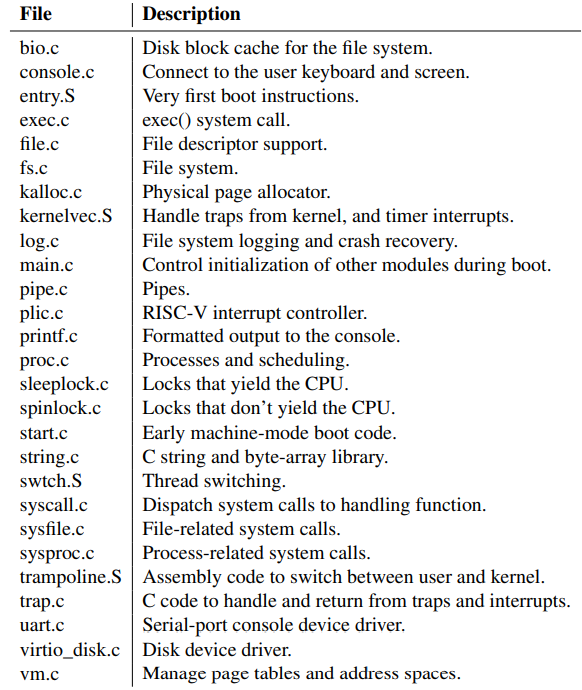
\includegraphics[width=0.5\textwidth]{figures/figura-xv6-1.png}
\centering
\caption{Archivos fuente del kernel de xv6 y sus funciones principales.}
\label{fig:figura_xv6_1}
\centering
\small Fuente: Obtenido de \citep{xv6_mit} \textit{xv6: a simple, Unix-like teaching operating system}.
\end{figure}


\subsection{Componentes implementados (procesos, memoria, archivos, etc.)}
XV6 implementa los componentes esenciales de un sistema operativo Unix clásico, adaptados a un entorno educativo. A continuación, se describen los principales subsistemas y su funcionamiento técnico (ver Tabla \ref{tab:xv6_componentes}).

\begin{table}[H]
\centering
\caption{Componentes principales del sistema operativo \textbf{XV6}}
\label{tab:xv6-componentes}
\begin{tabular}{|p{4cm}|p{4cm}|p{7cm}|}
\hline
\textbf{Componente / Subsistema} & \textbf{Archivo(s) principal(es)} & \textbf{Funcionamiento técnico (idea clave)} \\ \hline
Gestión de procesos y planificador & \texttt{proc.c}, \texttt{proc.h} & Define la estructura \texttt{proc} y el planificador round-robin por CPU; maneja el ciclo de vida de procesos (\texttt{fork}, \texttt{exec}, \texttt{exit}, \texttt{wait}). \\ \hline
Gestión de memoria virtual & \texttt{vm.c}, \texttt{kalloc.c} & Implementa tablas de páginas por proceso (Sv39) y asignador físico mediante \texttt{kalloc/kfree}. \\ \hline
Sistema de archivos & \texttt{fs.c}, \texttt{file.c}, \texttt{log.c} & FS tipo Unix con \texttt{inode}, directorios, caché de bloques y journaling mediante write-ahead log. \\ \hline
Interfaz de \texttt{syscalls} & \texttt{syscall.c}, \texttt{sysproc.c}, \texttt{usys.S} & Tabla de \texttt{syscalls} y despacho de traps del modo usuario al kernel (\texttt{fork}, \texttt{read}, \texttt{write}, etc.). \\ \hline
Sincronización & \texttt{spinlock.c}, \texttt{sleeplock.c} & Provee \texttt{spinlock} y \texttt{sleeplock} para exclusión mutua y bloqueos dormibles. \\ \hline
Entrada/Salida y drivers & \texttt{console.c}, \texttt{uart.c}, \texttt{virtio\_disk.c} & Drivers básicos UART y VirtIO integrados con la caché de bloques. \\ \hline
Programas de usuario y shell & \texttt{user/sh.c}, \texttt{user/*.c} & Shell simple y utilidades de usuario para probar \texttt{syscalls}. \\ \hline
\end{tabular}
\end{table}

\subsubsection*{Gestión de procesos y planificación}
En xv6, cada proceso representa una única unidad de ejecución con su propio hilo. Cada uno mantiene su contexto independiente (registros, tabla de páginas, etc.), que se guarda y restaura cuando el sistema cambia entre procesos. El kernel almacena toda esta información en una estructura por proceso, similar a otros sistemas Unix.\cite{xv6_mit}(pag.19)

La creación de procesos sigue el modelo tradicional: fork() genera un proceso hijo que es una copia del padre, mientras que exec() permite cargar un programa completamente nuevo. Todos los procesos comparten el mismo entorno básico, sin distinciones entre diferentes usuarios.
La planificación utiliza un algoritmo round-robin muy básico. Cada CPU tiene su propio planificador que recorre cíclicamente la lista de procesos listos para ejecutar, asignando a cada uno un turno de tiempo fijo. No existen prioridades ni políticas complejas, manteniendo el diseño deliberadamente simple.\cite{xv6_mit}(pag.82)
\subsubsection*{Gestión de memoria virtual}
Xv6 gestiona la memoria mediante paginación, donde cada proceso opera en su propio espacio de direcciones virtuales independiente. El hardware (específicamente RISC-V) se encarga de traducir estas direcciones virtuales a físicas usando tablas de páginas. Aunque RISC-V soporta direcciones de 64 bits, xv6 utiliza solo los 38 bits inferiores, lo que teóricamente permite a cada proceso acceder hasta aproximadamente 256 GB de memoria.\cite{xv6_mit}(pag.38)

El espacio de direcciones de cada proceso sigue la convención Unix clásica:
La distribución de la memoria sigue el diseño clásico de Unix:

\begin{itemize}
    \item \textbf{Segmento de Código}: Ubicado en las direcciones más bajas (cerca de 0), con permisos de solo lectura y ejecución para proteger el código del programa.
    
    \item \textbf{Datos y Heap}: Situados a continuación del código, con permisos de lectura y escritura. El heap puede expandirse dinámicamente cuando el programa solicita más memoria mediante la llamada \texttt{sbrk}.
    
    \item \textbf{Pila del Usuario}: Se encuentra en la parte superior del espacio de direcciones y crece hacia abajo. También tiene permisos de lectura y escritura. Para detectar desbordamientos, existe una ``página guardia'' justo debajo de la pila; si un programa intenta escribir en esta zona, el kernel intercepta el fallo y termina el proceso.
\end{itemize}

\begin{figure}[H]
\centering
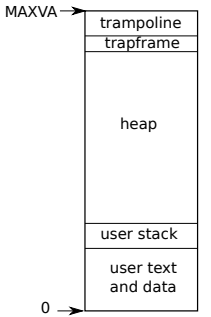
\includegraphics[width=0.5\textwidth]{figures/figura-xv6-2.png}
\centering
\caption{Layout del espacio de direcciones de un proceso xv6 . El proceso ve en su espacio un segmento de texto (solo lectura/ejecución), un segmento de datos/heap (lectura-escritura), y una pila de usuario (lectura-escritura hacia abajo)}
\label{fig:fig:figura_xv6_2}
\centering
\small Fuente: Obtenido de \citep{xv6_mit} \textit{xv6: a simple, Unix-like teaching operating system}.
\end{figure}

\subsubsection*{Sistema de archivos}
El sistema de archivos de xv6 organiza la información de forma jerárquica y utiliza journaling para garantizar la integridad de los datos. Su arquitectura sigue un diseño por capas similar a Unix, donde cada nivel se especializa en una función específica: desde el acceso físico al disco, pasando por la memoria caché de bloques, el registro transaccional, hasta la gestión de archivos, directorios y rutas. \citep{xv6_files_system}.

\textbf{Organización en Disco}
El disco se estructura en secciones bien definidas:

\begin{itemize}
    \item \textbf{Bloque 0}: Contiene el código de arranque
    \item \textbf{Bloque 1}: Almacena el ``superbloque'' con los metadatos del sistema de archivos
    \item \textbf{Bloques siguientes}: Albergan los inodos (que representan archivos)
    \item \textbf{Secciones posteriores}: Incluyen mapas de bits para espacios libres y los bloques de datos reales
    \item \textbf{Zona final}: Reservada para el journal o registro transaccional
\end{itemize}

\textbf{Mecanismo de Journaling}
Para prevenir corrupción de datos, xv6 emplea un sistema transaccional:

\begin{itemize}
    \item Antes de escribir cambios definitivos en el disco, estos se registran temporalmente en el journal
    \item Solo cuando la transacción se completa satisfactoriamente, los cambios se aplican permanentemente
    \item En caso de fallos (como cortes de energía), el sistema puede recuperar el estado coherente revisando el journal
\end{itemize}

\textbf{Gestión de Archivos y Directorios}
Los directorios son archivos especiales que contienen asociaciones entre nombres y inodos. El sistema resuelve las rutas de manera secuencial (por ejemplo, para \texttt{/usr/bin/ls}, busca primero \texttt{usr}, luego \texttt{bin}, y finalmente \texttt{ls}).

Las operaciones básicas (\texttt{open}, \texttt{read}, \texttt{write}, \texttt{close}) trabajan mediante descriptores de archivo. Internamente, estas llamadas utilizan la memoria caché de bloques: \texttt{read} carga bloques del disco a memoria, mientras \texttt{write} los marca como modificados para su posterior escritura transaccional.
\citep{xv6_mit}(pag. 85-86)

\subsubsection*{Interfaz de llamadas (syscalls)}
Xv6 implementa una interfaz de llamadas al sistema (syscalls) que permite a los programas de usuario solicitar servicios del kernel. Esta interfaz sigue el modelo tradicional de Unix, donde las llamadas al sistema son invocadas mediante interrupciones de software que cambian el modo de ejecución del CPU del modo usuario al modo kernel.\citep{xv6_mit}(pag.9)
Cuando un proceso de usuario realiza una syscall, el hardware genera una interrupción que transfiere el control al kernel. El kernel entonces identifica la syscall solicitada mediante un número único y despacha la ejecución a la función correspondiente en el kernel. Una vez que la syscall se completa, el kernel devuelve el control al proceso de usuario, junto con cualquier valor de retorno necesario.
\subsubsection*{Sincronización}
Xv6 proporciona mecanismos básicos de sincronización para gestionar el acceso concurrente a recursos compartidos. Los principales mecanismos son los \texttt{spinlocks} y \texttt{sleeplocks}.\citep{xv6_mit}(pag.65)

\subsubsection*{Entrada/Salida y drivers}
Los dispositivos en xv6 se integran en el sistema bajo el principio de que ``todo es un archivo''. Esto se logra mediante \textbf{archivos de dispositivo}, creados con la llamada al sistema \texttt{mknod}.

\begin{itemize}
    \item \texttt{mknod(path, major, minor)}: Crea un archivo especial que representa un dispositivo. Los parámetros \texttt{major} (mayor) y \texttt{minor} (menor) son números que identifican de forma única al controlador (\textit{driver}) del kernel y al dispositivo específico.
\end{itemize}

\textbf{Controladores de Dispositivos (Drivers)}
El kernel incluye controladores mínimos pero funcionales para hardware esencial. Algunos ejemplos son:

\begin{itemize}
    \item \texttt{uart.c} para el puerto serie.
    \item \texttt{virtio\_disk.c} para el acceso al disco.
    \item \texttt{timer.c} para el temporizador del sistema.
\end{itemize}

Xv6 prioriza la simplicidad, por lo que solo implementa los controladores estrictamente necesarios para el arranque y operación básica, sin soporte para red u otros periféricos complejos.

\subsubsection*{Programas de usuario y shell}
Xv6 incluye un shell básico inspirado en el Bourne shell, programado completamente en C. Este intérprete de comandos realiza las funciones esenciales: leer órdenes del usuario, soportar operaciones básicas como tuberías y redirecciones, y ejecutar programas creando nuevos procesos.
\textbf{Funcionamiento del shell}
Cuando introduces un comando como \texttt{ls | grep txt}, el shell:

\begin{itemize}
    \item Crea dos procesos hijos independientes
    \item Conecta la salida del primer proceso (\texttt{ls}) con la entrada del segundo (\texttt{grep}) mediante una tubería
    \item Espera a que ambos procesos terminen su ejecución
\end{itemize}

\subsection{Herramientas utilizadas (compiladores, emuladores, etc.)}
Para construir y ejecutar xv6 se emplean compiladores GNU y emuladores comunes. El código se compila con GCC (o clang compatibles) apuntando a binarios ELF para x86/RISC-V \citep{xv6_source}. En sistemas Unix/Linux se puede usar el compilador nativo; en macOS es necesario un cross-compiler para generar ELFpdos.csail.mit.edu. Normalmente se ejecuta en máquinas virtuales mediante QEMU como emulador de hardware.

\begin{table}[h]
\centering
\caption{Herramientas de desarrollo para xv6}
\begin{tabular}{|l|p{10cm}|}
\hline
\textbf{Herramienta} & \textbf{Uso / Descripción} \\
\hline
GCC (GNU C Compiler) & Compila el kernel y programas en C para x86-32 o RISC-V (binarios ELF). \\
\hline
QEMU & Emulador de hardware (Intel x86 o RISC-V) para cargar y probar xv6. \\
\hline
Cross-compiler & Necesario en macOS u otros sistemas para generar ejecutables ELF. \\
\hline
\end{tabular}
\end{table}

 \newpage
\subsection{Nivel de complejidad y accesibilidad para estudiantes}
Xv6 fue diseñado específicamente para ser un sistema operativo ligero y educativo. Su código completo consta de aproximadamente 10,000 líneas (equivalente a unas 99 páginas impresas)
Su simplicidad relativa (ausencia de capas complejas como módulos dinámicos) lo hace muy accesible para estudiantes de OS. Aun así, cubre los conceptos esenciales de concurrencia, paginación, sistemas de archivos y llamadas al sistema típicos de un Unix real\citep{xv6_mit} (pag.10)